<<<<<<< HEAD
\section{System design}\label{sec:systemdesign}
=======
\section{Design Goals and System Architecture}\label{sec:systemdesign}

In this part, we identify the design goals of $\DQV$ as a visualization system that supports fine-grained understanding of the query execution process and introduce its overall architecture.   
>>>>>>> 87e38476d46c232532b1981a1ff0ea0f46d2299d


\subsection{Requirement Analysis}
%During one year of collaboration, we have closely collaborated with three experts in distributed database, who are also the co-authors of this paper.
%
%In the first month of the collaboration, we have held brainstorming to collect the most frequent raised questions when analyzing the distributed query system performance. Based the discussions with domain experts and review of existing literature, we have formulated the following design requirements.

In the $\DQV$ project, we collaborated closely with three experts in distributed database systems, who are also co-authors of this paper. In the first month of the project, we brainstormed to collect the most frequently raised questions when analyzing the performance of distributed query processing. Based on these discussions and by reviewing existing literature, we identified the following design requirements for $\DQV$.

%\begin{itemize}
%  \item[\textbf{R1}]\textbf{Understand the general query execution progress and query plan structure.} Before our collaboration, the domain experts have used profiling software (Tez  UI, etc) or visualization tools(Tableau, etc) to show the query progress as Gantt chart and query plan structure as directed graph. However, these two visualizations are always displayed in separated views which require users to switch their focus thus break the continuity of exploration.
%  \item[\textbf{R2}]\textbf{Understand the query process at the task level.}Tez task is the atomic level of executions because ny failure operation in the task will lead to the re-run of whole task. Understand the execution of single task can be helpful to identify the bottleneck of the whole query process. However, visualize the tasks is challenge. First, to visualize the tasks in traditional way(Gantt chart) need a very large rendering space. Multiple features such as the size of input/output data and the operators should be visualized for understanding the task. Moreover, the many to many relationship among the tasks also makes it difficult to design clear and \textbf{scaleble} visualization.
%  \item[\textbf{R3}]\textbf{Provide the visual insight to reason the behaviour and pattern of a specific task.}To solely visualize the tasks themselves are not enough to explain the specific pattern of tasks. Many performance of hardware resource such as the network status, hard disk waiting list is also related to the patterns. Such kinds of information should be vitalized effectively to assist the exploration of query executions. 
%  \item[\textbf{R4}]\textbf{ Support interactive exploration.} Other than the visualization designs, a flexible interaction should be implemented for users to navigate to any time range, vertex, task group or single task of interest. The linkage among the correlated visual elements are also should be considered om the design to coordinate the information.
%\end{itemize}


\begin{itemize}
	\item[\textbf{R1}]\textbf{Understand the logical query plan and overall query execution progress.} Before our collaboration, the domain experts used profiling software (Tez  UI, etc) or visualization tools (Tableau, etc) to show the query plan as DAG and the query progress as Gantt chart. Although the two views help understanding query processing, the domain experts complained that they need to switch their focuses back and forth as the two views are separated, which breaks the continuity of exploration.
	
	\item[\textbf{R2}]\textbf{Understand query execution at the atom task level.} Task is the minimum execution unit in Tez and visualizing the execution of individual tasks is crucial for identifying the bottleneck of query processing. However, it is challenging to visualize the tasks. First, there are a large number of tasks and thus using traditional Gantt chart will require a very large rendering canvas. Rich information, such as input/output data size, start/finish time and involved operators, should be visualized alongside the tasks to facilitate understanding. Moreover, the many-to-many dependencies among the tasks make it difficult to design clear and \textbf{scalable} visualization.
	
	\item[\textbf{R3}]\textbf{Provide visual insights for reasoning query performance and correlating with system statuses.} $\DQV$ should make it easy to identify performance problems and conduct query optimization. Specifically, it should visualize the tasks in intuitive ways to support pinpointing suspicious tasks that may be the performance bottleneck. As system statuses such as network bandwidth and CPU load are also important for task execution, $\DQV$ should provide visualizations to connect task performance with system statistics. 
	
	\item[\textbf{R4}]\textbf{Support interactive exploration.} In addition to the visualization designs, $\DQV$ should provide flexible interaction mechanisms that allow users to navigate to any time range, DAG vertex, task group or individual task of interest. The linkage among correlated visual elements should also be considered in the design to coordinate information from different perspectives.
\end{itemize}

%\subsection{Task Analysis}
%Guided by the design requirements, we discussed with the domain experts about the visualizations $\DQV$ should provide and distilled the following visualization tasks:
%
%\begin{itemize}
%  \item[\textbf{T1}]\textbf{Visualize the query plan structure and execution process effectively.} To guarantee the continuity of exploration(R1), the process and plan structure should be integrated into one visualization view. Several criteria should be considered such as the minimize usage of canvas, minimize the cross of links and provide clear topology structure.
%  
%  \item[\textbf{T2}]\textbf{Effectively visualize the information of tasks.} To facilitate the fine grained exploration of query execution(\textbf{R1}, \textbf{R2}), the information about the tasks should be visualized, including: the size of data processed by the task; the data-flow among the tasks; the temporal information of task(start the time, end time, duration, etc) and the corresponding sub-process. Moreover, the abnormal(tasks taking longer time) tasks and the specific execution trace should be easily observed.
%  
%  \item[\textbf{T3}]\textbf{Visualize the machine status.} Display the machine status such as network status, disk IO pending list, CPU usage and Memory Usage will be useful to investigate the characters of task, and reasoning the patterns of the query execution( \textbf{R3}). These performance metrics should be well linked with the specific patterns of tasks. 
%  
%  \item[\textbf{T4}]\textbf{Interaction and linkage.} System should provide the flexible interactions allowing users to switch the focus among the different point of interest, such as a specific time range, a vertex or a group of tasks(\textbf{R2}, \textbf{R3}, \textbf{R4}). For example, user may select a vertex and explore if the tasks in this vertex are CPU-bound or I/O-bound. This requires the visualization to show the related tasks when choosing a vertex and highlight the corresponding CPU usage and disk information simultaneously.
%
%
%\end{itemize}


\subsection{Task Analysis}
Guided by the design requirements, we discussed with the domain experts about the visualizations $\DQV$ should provide and distilled the following visualization tasks:

\begin{itemize}
	\item[\textbf{T1}]\textbf{Jointly visualize the query plan and execution progress.} To ensure the continuity of exploration (R1), the logical query plan and query execution progress should be integrated into one visualization view. The visualization should meet several important criteria such as minimize the usage of canvas, reduce the number of links and show the task dependencies clearly.
	
	\item[\textbf{T2}]\textbf{Visualize comprehensive information about the tasks.} To facilitate fine-grained exploration of query execution (\textbf{R1}, \textbf{R2}), rich information about the tasks should be visualized, including the size of the data processed by each task, the data-flow among the tasks, the temporal information of individual tasks (start time, finish time, duration and etc.) and the corresponding sub-process. Moreover, the abnormal tasks (which may be the query bottleneck) and related execution traces should be easily observed.
	
	\item[\textbf{T3}]\textbf{Visualize the system statuses.} To investigate the system reasons behind task performance (\textbf{R3}), $\DQV$ should display the execution statistics of the overall system and each individual machine such as the amount of send/receive data, disk IO pending list, CPU usage and memory occupancy. These system statistics should be well linked with specific execution patterns of tasks. 
	
	\item[\textbf{T4}]\textbf{Interaction and linkage.} $\DQV$ should provide flexible interactions that allow users to switch their focuses between the different points of interest, such as a specific time range, a vertex or a group of tasks (\textbf{R2}, \textbf{R3}, \textbf{R4}). For example, a user may select a vertex in the logical plan and try to determine its tasks are CPU-bound or IO-bound. This requires the visualization to show the related tasks when choosing a vertex and highlight the corresponding CPU usage and disk information in a cohesive manner.
\end{itemize}


\subsection{System Architecture}
\begin{figure}[t]
	\centering
	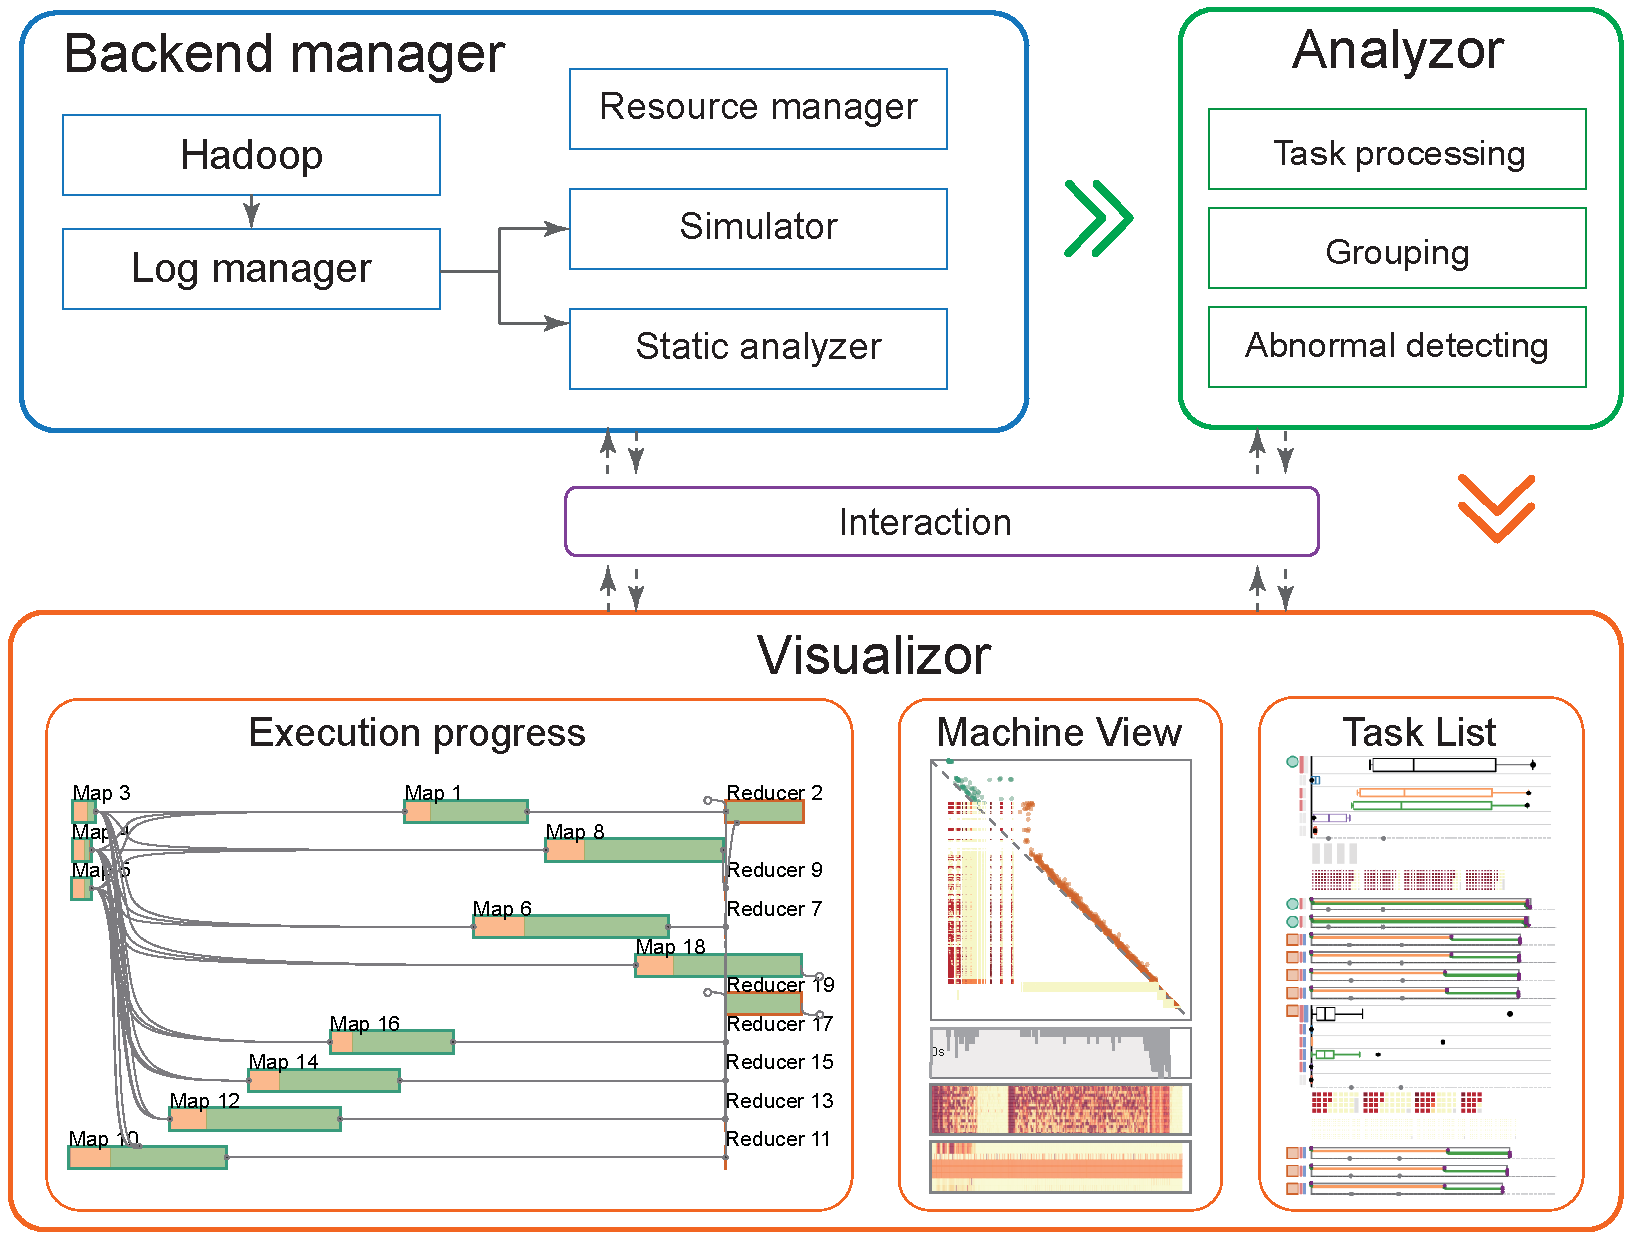
\includegraphics[width=0.45\textwidth]{figures/system/sysdesign.pdf}
	\vspace{-3mm}
	\caption{$\DQV$ system consists of three major components, i.e., backend manager, analyzer and visualizer.}
	\label{fig:sysdesign}
	\vspace{-3mm}
\end{figure}
%We use build $\DQV$ based on Hadoop2.0 with \textbf{Hive} as query optimizer and \textbf{Tez} as the executor. As shown by Figure~\ref{fig:sysdesign}, $\DQV$ consists of three modules: backend manager, analyzer, and visualizer. 
%
%
%The \textbf{Backend Manager} module performs the log processing and data fusion. Two categories of data are collected and fused: the execution data and the system performance data.
%When collecting the execution data from Hadoop system, the Log Manager cleans and preprocesses the log files, extracts the important metrics and saves them as the local files.
%Log analyzer directly takes these files as input and processes them as structured data for future processing.
%Monitor module segments the data at the specific time range and output them with a given rate.
%The simulator simulates the execution progress, allowing users to adjust the running speed and explore the dynamic query process.
%Moreover, Resource Manager collect the system performance metrics and output them to the next processing stage.
%
%
%The \textbf{Analyzer} fuses the execution data and system performance data by timestamps. The tasks will be grouped according to the vertex of the execution plan. The dataflow dependencies are recorded in this step. Moreover, Analyzor also performs the anomaly detection for the tasks in a group to enable the in-depth analysis.
%
%
%The \textbf{Visualizor} module integrates coordinated views to support interactive exploration of query execution results and reasoning about the query behavior at multiple levels. The Execution Overview demonstrates the execution process at the vertex level. An algorithm for the temporal DAG is proposed to visualize the structure and procedure simultaneously. The task group view consists of two components: 1) task overview visualizes the temporal information and data dependencies of tasks executed on the same machine; 2) metrics component shows the corresponding machine performance metrics. The task list view provides more detailed information at the operator level, enabling the users to understand and compare the time usage of tasks.


We build $\DQV$ on the top of Hadoop2.0 with \textbf{Hive} as the query optimizer and \textbf{Tez} as the executor. As shown in Figure~\ref{fig:sysdesign}, $\DQV$ consists of three modules: backend manager, analyzer, and visualizer. 


The \textbf{Backend Manager} module performs log processing and data fusion for query execution data and system performance data. When collecting execution data from the Hadoop system, the Log Manager cleans and pre-processes the log files, extracts important metrics and saves them as local files.
Log Analyzer takes these files as input and processes them as structured data for future processing.
Monitor segments the data at regular time ranges and output them at a given rate.
The Simulator simulates the query execution process, and allows users to adjust the running speed and explore the execution process interactively.
Moreover, Resource Manager collects system performance metrics and outputs them to the next processing stage.


The \textbf{Analyzer} fuses the execution data and system performance data by timestamps. The tasks will be grouped according to their corresponding vertices in the logical execution plan. The dataflow among the tasks (i.e., dependencies) are also recorded in this step. Moreover, Analyzer also performs the anomaly detection for the tasks to support in-depth analysis.


The \textbf{Visualizer} module integrates coordinated views to support interactive exploration of the query execution process and reasoning about query performance from multiple levels. The Execution Overview demonstrates the execution process at the vertex level. An algorithm for temporal DAG layout is proposed to visualize the structure of the logical execution plan and the query execution progress simultaneously. The task group view consists of two components: (i) task overview, which
visualizes the temporal information and data dependencies of the tasks executed on the same machine, and (ii) system statuses, which shows the performance statistics of the corresponding machine. The task list view provides more detailed information at the operator level, enabling the users to analyze the execution statistics of individual tasks.  

